\documentclass{beamer}

\mode<presentation>
{
  \usetheme{Antibes}
  \usecolortheme{beaver}
  % or ...

  \setbeamercovered{transparent}
  % or whatever (possibly just delete it)
}


\usepackage[english]{babel}
\usepackage[utf8]{inputenc}
\usepackage{times}
\usepackage[T1]{fontenc}
\usepackage{graphicx}
\usepackage[compatibility=false]{caption}
\usepackage{subcaption}
\usepackage{physics}
\usepackage{amsmath}
\usepackage{amssymb}

%\usepackage{multimedia}
%\usepackage{movie9}


\newcommand{\expv}[1]{\ensuremath{\mathbb{E}[ #1]}}
\newcommand{\xs}[2]{\ensuremath{\Sigma_{#1}^{(#2)}}}
\newcommand{\intO}{\ensuremath{\int\limits_{4\pi}}}
\newcommand{\intz}{\ensuremath{\int\limits_0^1}}
\newcommand{\intf}{\ensuremath{\int\limits_{-\infty}^\infty}}
\newcommand{\intzf}{\ensuremath{\int\limits_{0}^\infty}}

\title[UQ in RAVEN] % (optional, use only with long paper titles)
{Advanced Methods in \\Stochastic Collocation for Polynomial Chaos\\in RAVEN}

%\subtitle
%{A Term Project}

\author[Talbot] % (optional, use only with lots of authors)
{Paul W. Talbot}%\inst{1}}


\institute[University of New Mexico] % (optional, but mostly needed)
{
  %\inst{1}%
  University of New Mexico%\\
  %\inst{2}
  %Idaho National Laboratory
}

\date[Jan 22 2016] % (optional, should be abbreviation of conference name)
{Dissertation Proposal, January 22nd 2016\\\vspace{10pt}\small Funded by a Laboratory Directed Research effort at Idaho National Laboratory}


\subject{Uncertainty Quantification}

\pgfdeclareimage[height=0.5cm]{university-logo}{../../graphics/unmlogo}
%\logo{\pgfuseimage{university-logo}}
\logo{\makebox[0.95\paperwidth]{
  
\includegraphics[height=1cm]{../../graphics/INL}\hfill
    
\includegraphics[height=0.5cm]{../../graphics/unmlogo}}

}

\addtobeamertemplate{navigation symbols}{}{
  \usebeamerfont{footline}%
  \usebeamercolor[fg]{footline}%
  \hspace{1em}%
  \insertframenumber/\inserttotalframenumber
}

\makeatletter
\def\beamer@tocaction@only#1{\only<.(1)>{\usebeamertemplate**{#1}}}
\define@key{beamertoc}{subsectionsonly}[]{\beamer@toc@subsectionstyle{show/only}\beamer@toc@subsubsectionstyle{show/shaded/hide}}
\makeatother

\setbeamercovered{invisible}

\begin{document}
\AtBeginSection[]{\begin{frame}{Outline}\vspace{-20pt}
  \tableofcontents[currentsection,hideothersubsections]%,subsectionsonly]
\end{frame}}
%\AtBeginSection[]{\begin{frame}{Outline}
%  \tableofcontents[subsectionsonly,pausesections]
%\end{frame}}

\begin{frame}
  \titlepage
\end{frame}

%%%%%%%%%%%%%%%%%%%%%%%%%
%        OUTLINE        %
%%%%%%%%%%%%%%%%%%%%%%%%%

\begin{frame}{Outline}{Discussion Points}
  \begin{columns}
  \begin{column}{0.1\textwidth}
  \end{column}
  \begin{column}{0.9\textwidth}
    \setcounter{tocdepth}{2}
    \tableofcontents[]
  \end{column}
  \end{columns}
\end{frame}
%\begin{frame}{Outline}{Discussion Points}\vspace{-20pt}
%  \tableofcontents[hideallsubsections]%[pausesections]
  % You might wish to add the option [pausesections]
%\end{frame}

%%%%%%%%%%%%%%%%%%%%%%%%%%%%
%        BACKGROUND        % 10 minutes
%%%%%%%%%%%%%%%%%%%%%%%%%%%%
\section{Background}

\subsection{Terminology}
% describe uq in general
% introduce terminology
\begin{frame}{Background}{Terminology}\vspace{-20pt}
  \begin{itemize}
  \item Model - Mathematical representation
  \item Simulation/Code - Algorithms to Solve Model
  \item Output - Solution to Model \vspace{20pt}
  \item Input Space - Space Spanning Possible Input Values
  \item Response - Map of Input Space to Output Space
  \end{itemize}
\end{frame}

\begin{frame}{Background}{UQ}\vspace{-20pt}
  Understanding Simulations
  \pause
  \begin{itemize}
    \item Verification - Is the code consistent?
      \begin{itemize}
        \item Spatial, Temporal Convergence
      \end{itemize}\vspace{10pt}
    \item Validation - Does it match experiment?
      \begin{itemize}
        \item Fitting, Extrapolation
      \end{itemize}\vspace{10pt}
    \item Uncertainty Quantification - Behavior of Response
      \begin{itemize}
        \item Response Surface Characterization
      \end{itemize}
  \end{itemize}
\end{frame}

\begin{frame}{Background}{Verification and Validation}
  \vspace{-50pt}
  \begin{figure}[h!]
    \centering
      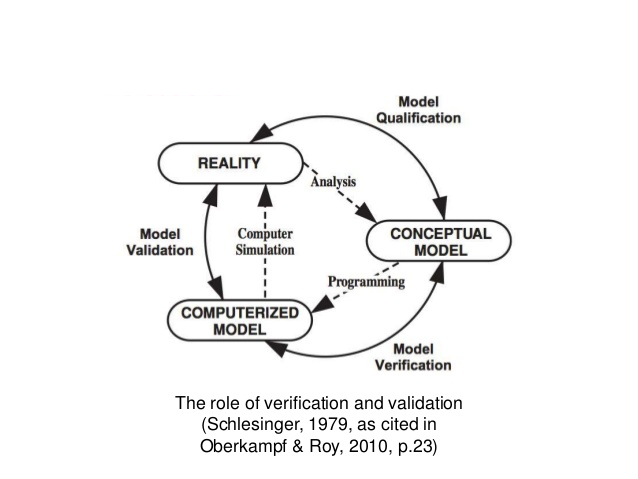
\includegraphics[width=0.8\textwidth]{../../graphics/v_and_v_1}
  \end{figure}
\end{frame}

\begin{frame}{Background}{Uncertainty Quantification}
  \vspace{-20pt}
  \begin{figure}[h!]
    \centering
      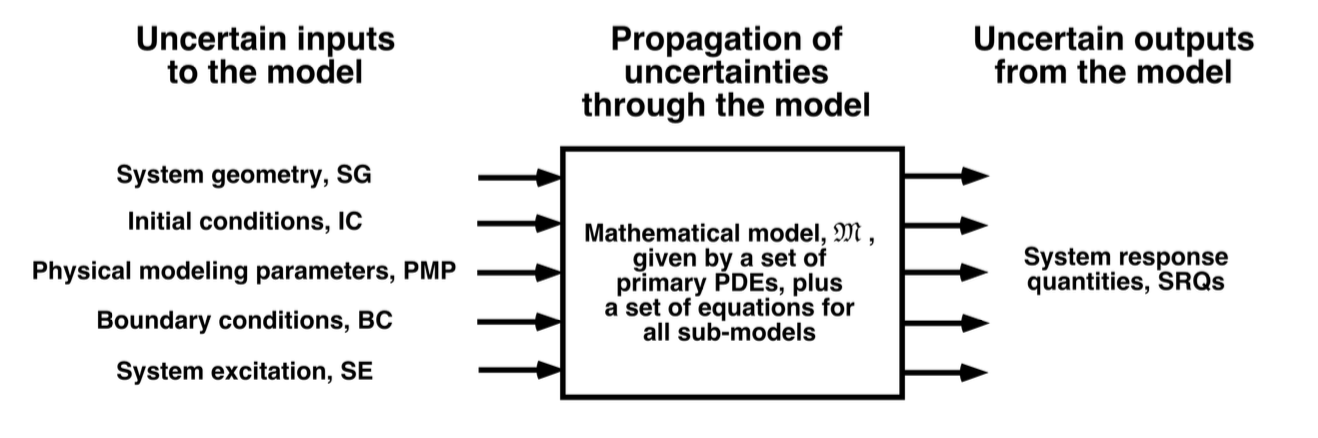
\includegraphics[width=0.8\textwidth]{../../graphics/v_and_v_uq}
  \end{figure}
  \hfill Oberkampf and Roy, 2010
\end{frame}


\subsection{Raven}
\begin{frame}{Background}{RAVEN}\vspace{-20pt}
  \begin{columns}
    \begin{column}{0.8\linewidth}
  \begin{itemize}
    \item (R)isk (A)nalysis (V)irtual (EN)vironment
    \item Verification and Validation
    \item Uncertainty Quantification
    \item Response Surfaces, Risk
    \item Reduced-Order Models
    \item Operates on Black-box Models
  \end{itemize}
    \end{column}
    \begin{column}{0.2\linewidth}
    \begin{figure}[h!]
      \centering
        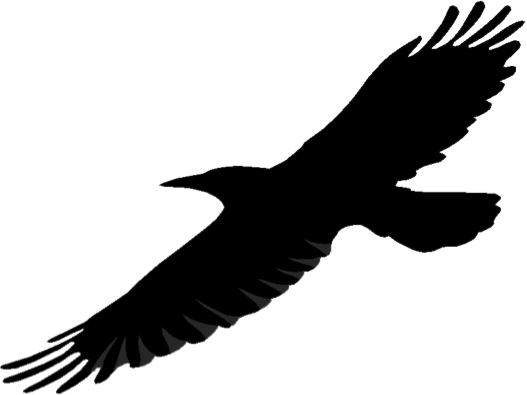
\includegraphics[width=\textwidth]{../../graphics/raven}
      \end{figure} \vspace{-20pt}
    \end{column}
  \end{columns}\vspace{10pt}
  Goal: Add New UQ Methods to RAVEN
\end{frame}

\subsection{Intrusiveness}
% Galerkin/Adjoint methods vs non-intrusive
\begin{frame}{Background}{Intrusiveness}\vspace{-20pt}
  Two approaches to UQ:\vspace{10pt}
  \begin{itemize}
    \item Intrusive
       \begin{itemize}
         \item Interacts with Simulation Algorithms
         \item Example: Adjoint-Based
       \end{itemize}
    \item Non-Intrusive
      \begin{itemize}
        \item Agnostic of Code
        \item Example: Monte Carlo
      \end{itemize}
  \end{itemize}\vspace{10pt}
  For RAVEN, need non-intrusive algorithms
\end{frame}

\subsection{Sampling Strategies}
\begin{frame}{Sampling Strategies}{Non-Intrusive Sampling Strategies}
  \vspace{-20pt}
  \begin{columns}
  \begin{column}{0.6\textwidth}
  Monte Carlo
    \begin{itemize}
      \item Generate independent, identically-distributed samples
      \item Derive mean, variance, response surface
    \end{itemize}
  Latin Hypercube
    \begin{itemize}
      \item Distributed Monte Carlo
    \end{itemize}
  \end{column}
  \begin{column}{0.4\textwidth}
    \begin{figure}[h!]
      \centering
        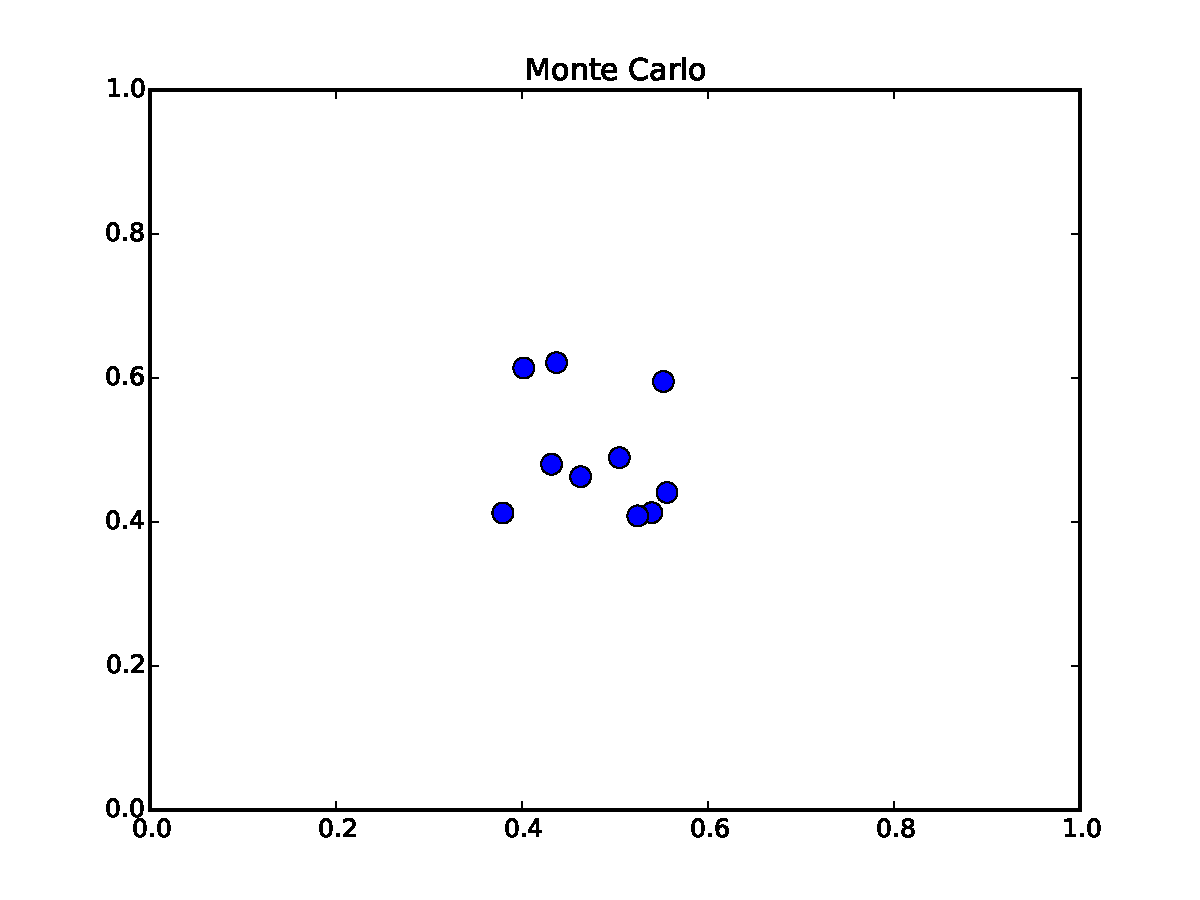
\includegraphics[width=\textwidth]{../../graphics/mc}
      \end{figure} \vspace{-20pt}
    \begin{figure}[h!]
      \centering
        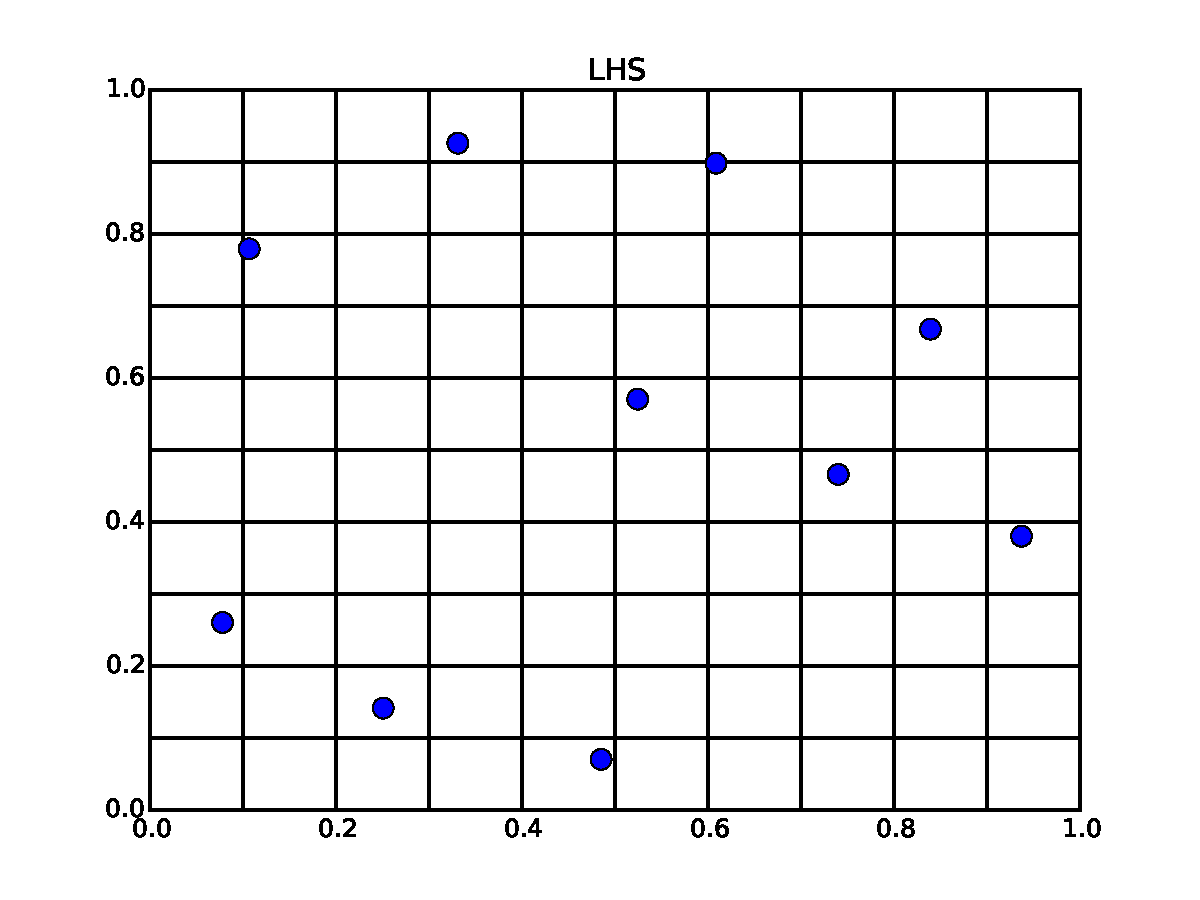
\includegraphics[width=\textwidth]{../../graphics/lhs}
    \end{figure}
  \end{column}
  \end{columns}
\end{frame}
% Monte Carlo and LHS
% gPC

\begin{frame}{Sampling Strategies}{Limitations}\vspace{-20pt}
  Monte Carlo common choice for UQ\vspace{10pt}
  \begin{itemize}
    \item Pro: Convergence agnostic of dimensionality
    \item Con: Convergence can take many, many samples
  \end{itemize}
\end{frame}

%%%%%%%%%%%%%%%%%%%%%%%%%%%%
%         METHODS          % 20-30 minutes
%%%%%%%%%%%%%%%%%%%%%%%%%%%%
\section{Methods}
%\begin{frame}{Methods}{Outline}\vspace{-20pt}
%  \tableofcontents[currentsection,hideothersubsections]%,subsectionsonly]
%\end{frame}


\subsection{UQ Methods}
\begin{frame}{Definitions}{}\vspace{-20pt}
  \begin{itemize}
    \item $N\in\mathbb{N^+}$ - Cardinality of Input Space
    \item Probabilty Space $(\Omega,\Theta,\rho)$, $Y:\Theta\to\mathbb{R}^N$
    \item $Y=(y_1,\cdots,y_N)$ - Uncertain Input Parameter Vector
    \item Subspaces $(\Omega_n,\Theta_n,\rho_n)$
    \item $Y\in\mathbb{R}^N$, $y_n\in\mathbb{R}\forall n\leq N,n\in\mathbb{N^+}$
    \item Members of $Y$ are uncorrelated
    \item $\rho(Y)=\prod_{n=1}^N \rho_n(y_n)$ - Joint Probability Density Function
    \vspace{10pt}
    \item $u(Y)$ - QoI as a function of Input Parameters $Y$
  \end{itemize}
\end{frame}


\subsubsection{SC for gPC}
\begin{frame}{Generalized Polynomial Chaos}{gPC}\vspace{-20pt}
  \begin{equation*}
    u(Y) = \sum_{k\in\Lambda} c_k \Phi_k(Y),
  \end{equation*}\vspace{-10pt}
  \begin{itemize}
    \item $\Lambda$ - a finite set of polynomial indices,
    \item $k=(k_1,\cdots,k_N)$ indexes $\Lambda$, $k_n\in\mathbb{N}^0$,
    \item $c_k\in\mathbb{R}$ - scalar coefficients,
    \item $\phi_{k_n}(y_n)$ - Gauss polys order $k_n$ orthonormal w.r.t $\rho_n(y_n)$,
    \item $\Phi_k(Y)=\prod_{n=1}^N\phi_{k_n}(y_n)$,
    \item $\Phi_k(Y)$ orthonormal w.r.t $\rho(Y)$ over $\Omega$.
  \end{itemize}
\end{frame}

\begin{frame}{Generalized Polynomial Chaos}{Truncated}\vspace{-20pt}
  In practice, truncate to some gPC level $L\in\mathbb{N^+}$,
  \begin{equation*}
    u(Y)\approx G_L[u](Y) \equiv \sum_{k\in\Lambda(L)} c_k \Phi_k(Y).
  \end{equation*}%\vspace{-10pt}
  Error is of order equal to the polynomial terms removed by truncation.
\end{frame}

\subsubsection{Polynomial Index Sets}
\begin{frame}{Generalized Polynomial Chaos}{Constructing $\Lambda(L)$}\vspace{-20pt}
  $\Lambda(L)$ is list of multidimensional polynomial indices $k$\vspace{25pt}\\
  For example, $N=3$:
  \begin{equation*}
    k = (3,1,2)\hspace{10pt}\to\hspace{10pt} \Phi_k(Y) = \phi_3(y_1)\phi_1(y_2)\phi_2(y_3).
  \end{equation*}
\end{frame}

\begin{frame}{Generalized Polynomial Chaos}{Constructing $\Lambda(L)$}%\vspace{-20pt}
  Na{\"i}ve choice for $\Lambda(L)$ is tensor product of all polynomials of order less than or equal to $L$,
  \begin{equation*}
      \Lambda_\text{TP}(L)=\Big\{k=(k_1,\cdots,k_N): \max_{1\leq n\leq N}k_n\leq L\Big\}.
  \end{equation*}
  Size of Index Set: $|\Lambda_\text{TP}(L)|=(L+1)^N$.
  \begin{table}[h]
    \centering
    \begin{tabular}{c c c c}
    (3,0) & (3,1) & (3,2) & (3,3) \\
    (2,0) & (2,1) & (2,2) & (2,3) \\
    (1,0) & (1,1) & (1,2) & (1,3) \\
    (0,0) & (0,1) & (0,2) & (0,3)
    \end{tabular}
    \caption{Tensor Product Index Set, $N=2,L=3$}
    \label{tab:TP}
  \end{table}
\end{frame}

\begin{frame}{Generalized Polynomial Chaos}{Constructing $\Lambda(L)$}%\vspace{-20pt}
  Common choice for $\Lambda(L)$: Total Degree of all polynomials of order less than or equal to $L$,
  \begin{equation*}
    \Lambda_\text{TD}(L)=\Big\{\bar p=(p_1,\cdots,p_N):\sum_{n=1}^N p_n \leq L\Big\}.
  \end{equation*}
  Size of Index Set: $|\Lambda_\text{TD}(L)|={L+N\choose N}$.
  \begin{table}[h]
    \centering
    \begin{tabular}{c c c c}
    (3,0) &       &       &       \\
    (2,0) & (2,1) &       &       \\
    (1,0) & (1,1) & (1,2) &       \\
    (0,0) & (0,1) & (0,2) & (0,3)
    \end{tabular}
    \caption{Total Degree Index Set, $N=2,L=3$}
    \label{tab:TD}
  \end{table}
\end{frame}

\begin{frame}{Generalized Polynomial Chaos}{Constructing $\Lambda(L)$}%\vspace{-20pt}
  Hyperbolic Cross: Limited by product of all polynomial orders,
  \begin{equation*}
    \Lambda_\text{HC}(L)=\Big\{\bar p=(p_1,\ldots,p_N):\prod_{n=1}^N p_n+1 \leq L+1\Big\}.
  \end{equation*}
  Index Set Bound: $|\Lambda_\text{HC}(L)|\leq (L+1)(1+\log(L+1))^{N-1}$.
  \begin{table}[h]
    \centering
    \begin{tabular}{c c c c}
    (3,0) &       &       &       \\
    (2,0) &       &       &       \\
    (1,0) & (1,1) &       &       \\
    (0,0) & (0,1) & (0,2) & (0,3)
    \end{tabular}
    \caption{Hyperbolic Cross Index Set, $N=2,L=3$}
    \label{tab:HC}
  \end{table}
\end{frame}

\begin{frame}{Generalized Polynomial Chaos}{Constructing $\Lambda(L)$}%\vspace{-20pt}
  Anisotropic Rules using weights $\alpha = (\alpha_1,\cdots,\alpha_N)$
  \begin{equation*}
    \tilde\Lambda_\text{TD}(L)=\Big\{\bar p=(p_1,\cdots,p_N):\sum_{n=1}^N \alpha_n p_n \leq \qty|\alpha|_1 L
  \Big\},
  \end{equation*}
  \begin{equation*}
    \tilde\Lambda_\text{HC}(L)=\Big\{\bar p=(p_1,\cdots,p_N):\prod_{n=1}^N \qty(p_n+1)^{\alpha_n} \leq
    \qty(L+1)^{\qty|\alpha|_1} \Big\}.
  \end{equation*}
  \begin{equation*}
    |\alpha|_1 \equiv \frac{\sum_{n=1}^N \alpha_n}{N}.
  \end{equation*}
\end{frame}


\subsubsection{Sparse Grid Quadrature}
\begin{frame}{Generalized Polynomial Chaos}{Sparse Grid Quadrature}%\vspace{-20pt}
  \pause
  Necessary to find coefficients $c_k$,
  \begin{equation*}
    G[u](Y) = \sum_{k\in\Lambda(L)} c_k \Phi_k(Y).
  \end{equation*}%\vspace{-10pt}
  Using orthonormality of $\Phi_k(Y)$,
  \begin{equation*}
    c_k = \langle u(Y)\Phi_k(Y) \rangle = \int_\Omega \rho(Y) u(Y)\Phi_k(Y) dY
  \end{equation*}
\end{frame}

\begin{frame}{Generalized Polynomial Chaos}{Sparse Grid Quadrature}%\vspace{-20pt}
  The quadrature and polynomials to use depends on the distribution $\rho_n(y_n)$,
  \begin{table}[h]
    \centering
    \begin{tabular}{c|c}
      PDF Kind & Polynomials / Quadrature \\ \hline
      Uniform & Legendre \\
      Normal  & Hermite  \\
      Gamma   & Laguerre \\
      Beta    & Jacobi   
    \end{tabular}
  \end{table}
\end{frame}

\begin{frame}{Generalized Polynomial Chaos}{Order of Quadrature}%\vspace{-20pt}
  Determine order of quadrature
  \begin{equation*}
    \int_{\Omega_x} f(x)\rho(x)dx = \sum_{\ell=1}^\infty w_\ell f(x_\ell).
  \end{equation*}
  If $f(x)$ is a polynomial of order $2m-1$,
  \begin{equation*}
    \int_{\Omega_x} f(x)\rho(x)dx = \sum_{\ell=1}^m w_\ell f(x_\ell).
  \end{equation*}
  Let
  \begin{equation*}
    q^{m}[f(x)] \equiv \sum_{\ell=1}^m w_\ell f(x_\ell).
  \end{equation*}
  In our case (let $N$=1),
  \begin{equation*}
    c_k = \int_{\Omega} u(Y)\Phi(Y)\rho(Y)dY = q^m[u(Y)\Phi(Y)].
  \end{equation*}
  Unknown $m$.
\end{frame}

\begin{frame}{Generalized Polynomial Chaos}{Order of Quadrature}\vspace{-20pt}
  \begin{equation*}
    c_k = \int_{\Omega} u(Y)\Phi(Y)\rho(Y)dY = q^m[u(Y)\Phi_k(Y)].
  \end{equation*}
  To determine $m$, replace $u(Y)=G[u](Y)$:
  \begin{align*}
    c_k &= q^m\left[\Phi_k(Y)\sum_{k'\in\Lambda(L)}c_{k'}\Phi_{k'}(Y)\right], \\
        &= q^m\left[c_k\Phi_k(Y)^2\right],\\
        &= q^m\left[\mathcal{O}(k^2)\right],
  \end{align*}
  so
  \begin{equation*}
    2m+1 = 2k \hspace{10pt}\to\hspace{10pt}m=k+\frac{1}{2}\approx m=k+1.
  \end{equation*}
\end{frame}

\begin{frame}{Generalized Polynomial Chaos}{Sparse Grid Quadrature}\vspace{-20pt}
  Multidimensional Quadrature
  \begin{itemize}
    \item Each point needs $N$ quadrature sets
    \item Ex. $N=2$, $k$=(4,4), need (5,5) quadratures
    \item Needed for each $k$ in $\Lambda$
  \end{itemize}
  \begin{columns}
  \begin{column}{0.6\linewidth}
  Tensor quadrature
  \begin{align*}
    Q^{M} &\equiv q^{m_1}_1 \otimes q^{m_2}_2 \otimes \cdots \otimes q^{m_N}_N,\\
                       &= \bigotimes_{n=1}^N q^{m_n}_n.
  \end{align*}
  \end{column}
  \begin{column}{0.4\linewidth}
    \begin{figure}[h!]
      \centering
        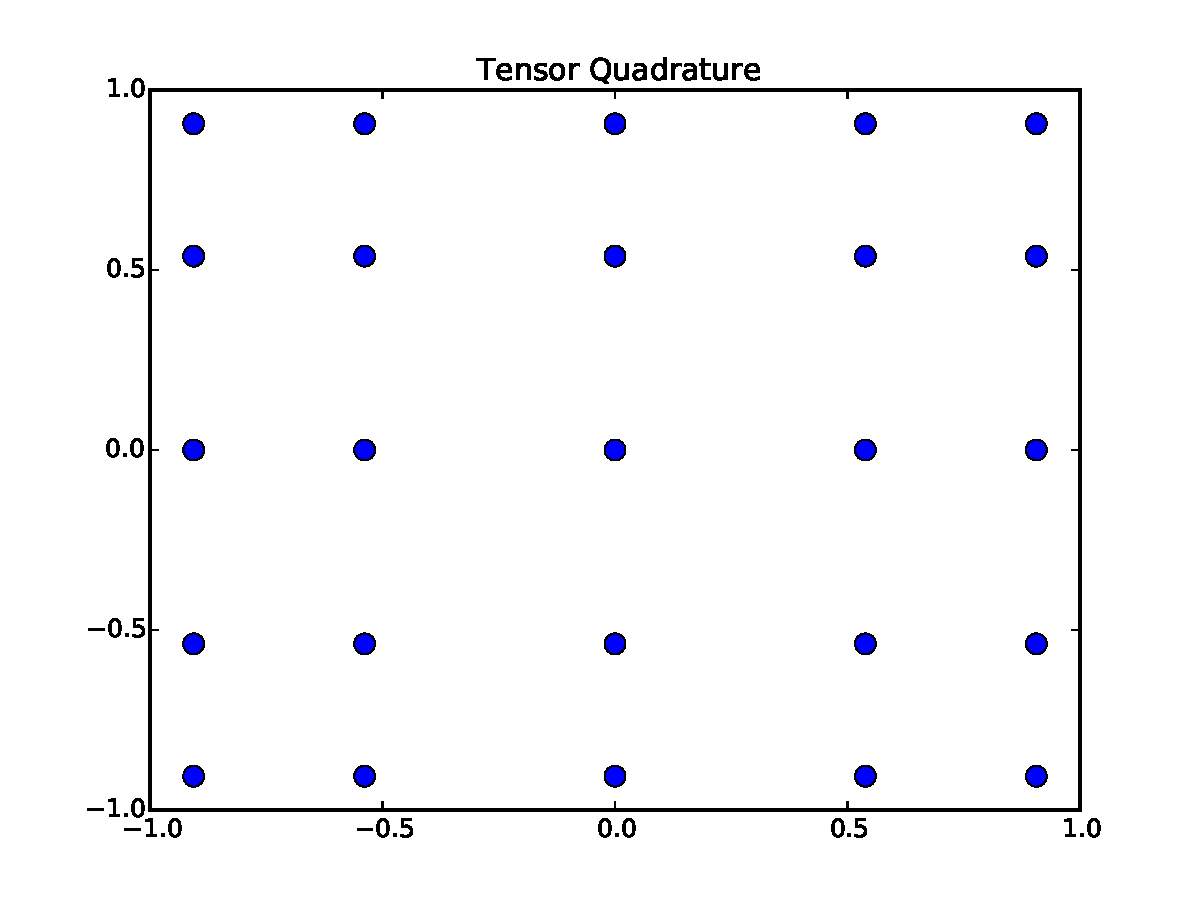
\includegraphics[width=\textwidth]{../../graphics/tpquad}
    \end{figure}
  \end{column}
  \end{columns}
\end{frame}

\begin{frame}{Generalized Polynomial Chaos}{Sparse Grid Quadrature}\vspace{-20pt}
Smolyak sparse grids $S[u](Y)$:
\begin{equation*}
  \text{Let }\Delta_k^{m}[f(x)] \equiv \qty(q_k^{m} - q_{k-1}^{m})[f(x)].
\end{equation*}
\vspace{10pt}
\begin{equation*}
  S^{M}_{\Lambda,N}[u(Y)\Phi_k(Y)] = \sum_{k\in\Lambda(L)} \left(\Delta_{k_1}^{m_1} \otimes \cdots \otimes
  \Delta_{k_N}^{m_N}\right)[u(Y)\Phi_k(Y)].
\end{equation*}
\end{frame}

\begin{frame}{Generalized Polynomial Chaos}{Sparse Grid Quadrature}%\vspace{-20pt}
  Equivalently,
\begin{equation*}
  S^{M}_{\Lambda,N}[u(Y)\Phi_k(Y)] = \sum_{k\in\Lambda(L)} s(k)\bigotimes_{n=1}^N
  q^{m_n}_n[u(Y)\Phi_k(Y)],
\end{equation*}
\begin{equation*}
  s(k) = \sum_{\substack{j=\{0,1\}^N,\\k+j\in\Lambda}} (-1)^{|j|_1},\hspace{10pt}|j|_1 \equiv \sum_{p\in j}p.
\end{equation*}
\begin{align*}
  c_k &= \langle u(Y)\Phi_k(Y) \rangle,\\
      &\approx S^{M}_{\Lambda,N}[u(Y)\Phi_k(Y)].
\end{align*}
\end{frame}

\begin{frame}{Generalized Polynomial Chaos}{Sparse Grid Quadrature}%\vspace{-20pt}
Comparison, $N=2$, $L=4$
    \begin{figure}[h!]
      \centering
       \hspace{-40pt}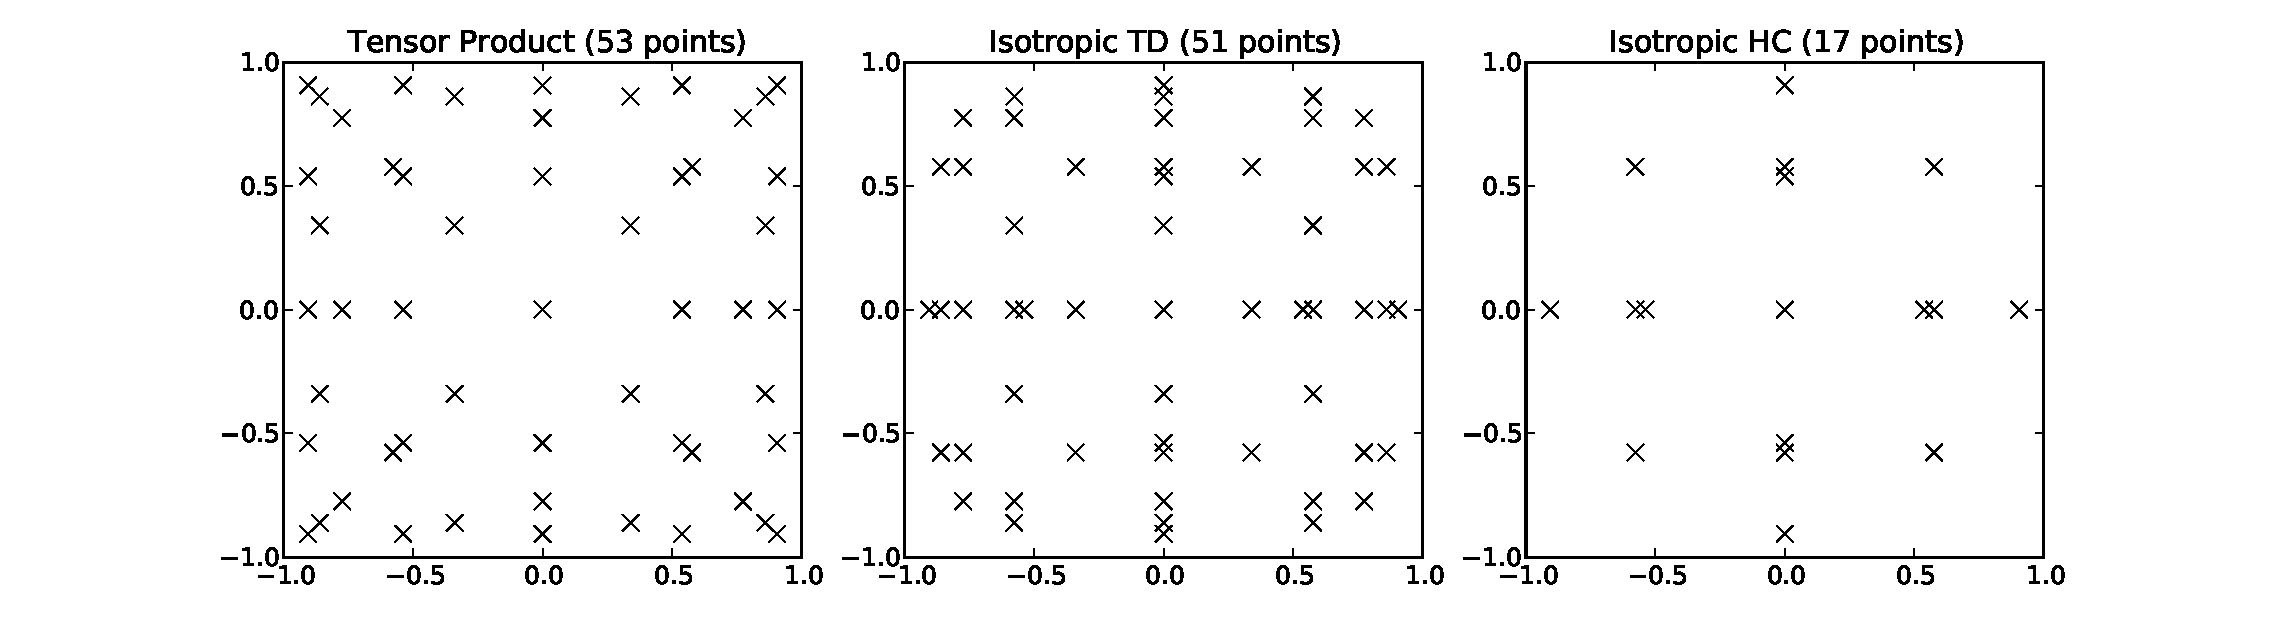
\includegraphics[width=1.15\textwidth]{../../graphics/sparse_plot}
    \end{figure}
\end{frame}

\subsubsection{Adaptive Sparse Grid}
\begin{frame}{Generalized Polynomial Chaos}{Adaptive Index Sets}%\vspace{-20pt}
  \pause
Special property of gPC:
\begin{equation*}
  G[u](Y) = \sum_{k\in\Lambda}c_k\Phi_k(Y),
\end{equation*}
\begin{equation*}
  \text{mean}=\langle G[u](Y)\rangle = c_{\{0\}^N},
\end{equation*}
\begin{align*}
  \text{var} &=\langle G[u](Y)^2\rangle - c_{\{0\}^N}^2,\\
      &= \sum_{k\in\Lambda}c_k^2 - c_{\{0\}^N}^2.
\end{align*}
\end{frame}

\begin{frame}{Generalized Polynomial Chaos}{Adaptive Index Sets}%\vspace{-20pt}
  Adaptive Index Set construction using ANOVA
  \begin{align*}
    \text{Impact Parameter }\eta_k &=
    \frac{c_k^2}{\text{var}\left\{G[u](Y)\right\}},\hspace{10pt}0\leq\eta_k\leq 1\\
    \text{Est. Impact Parameter }\tilde\eta_k &= \prod_{n=1,k_n>0}^N \eta_{(k_1,\cdots,k_n-1,\cdots,k_N)}
  \end{align*}
  Example,
  \begin{equation*}
    \tilde\eta_{(2,1,3)}=\eta_{(1,1,3)}\cdot\eta_{(2,0,3)}\cdot\eta_{(2,1,2)}
  \end{equation*}
\end{frame}

\begin{frame}{Generalized Polynomial Chaos}{Adaptive Index Sets}%\vspace{-20pt}
  Adaptive Index Set Algorithm
  \begin{itemize}
    \item Calculate mean (zeroth-order) polynomial expansion
    \item While not converged:
      \begin{itemize}
        \item Collect list of indices whose predecessors are in $\Lambda$
        \item Using existing impacts, predict impact of each potential index
        \item If total of impacts is less than tolerance, convergence is reached
        \item Otherwise, add highest-impact index and construct new expansion
      \end{itemize}
  \end{itemize}
\end{frame}

\begin{frame}{Generalized Polynomial Chaos}{Adaptive Index Sets}%\vspace{-20pt}
 \begin{figure}[h!]
   \centering
   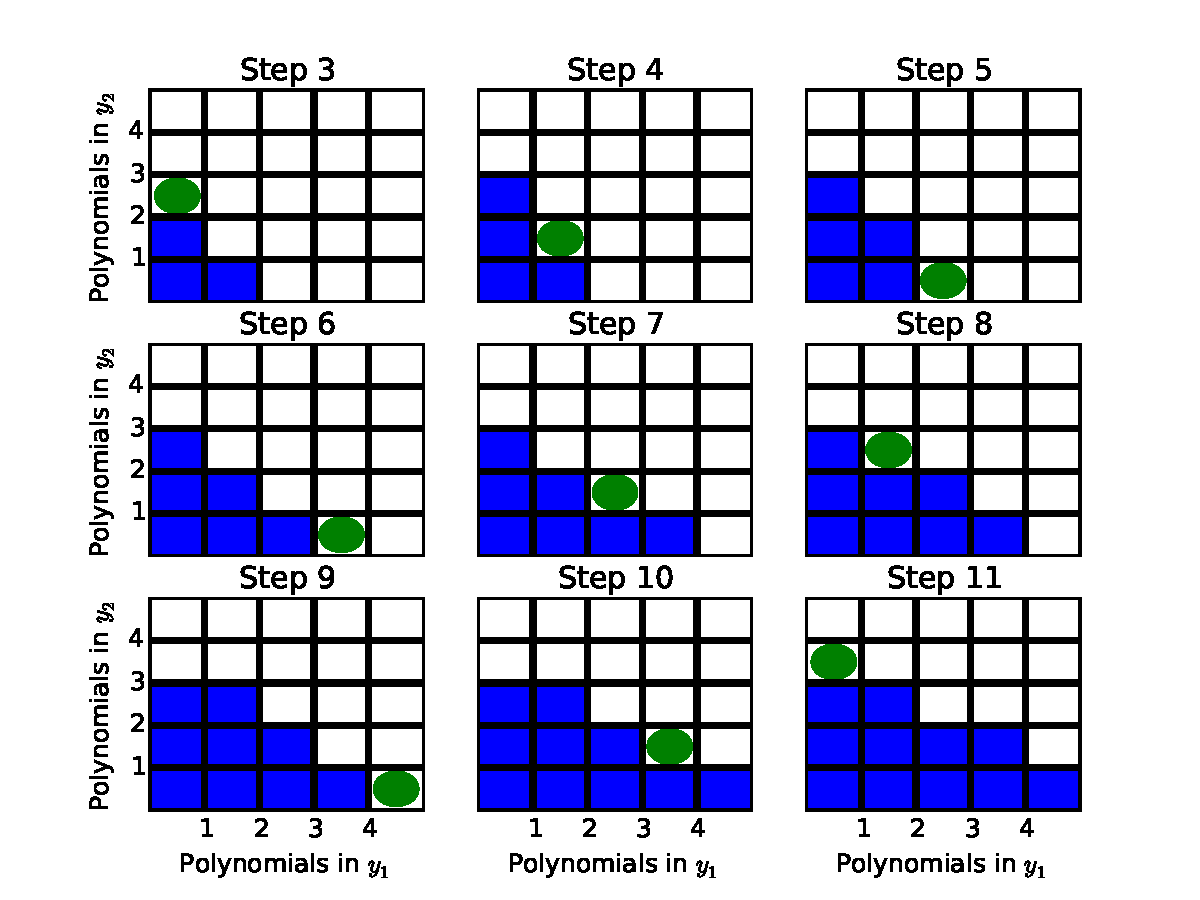
\includegraphics[width=0.8\textwidth]{../../graphics/asc_block}
 \end{figure}
\end{frame}

\subsection{Physics Models}
\begin{frame}{Physical Models}{}\vspace{-20pt}
  \pause
  Efficiency of gPC compared to Monte Carlo depends on
  \begin{itemize}
    \item Regularity of response surface
    \item Dimensionality of input space
  \end{itemize}\vspace{20pt}
  Demonstrate using three models
  \begin{itemize}
    \item Tensor Polynomial
    \item Attenuation
    \item Neutron Diffusion
  \end{itemize}
\end{frame}

\subsubsection{Tensor Polynomials}
\begin{frame}{Physical Models}{Tensor Polynomial}%\vspace{-20pt}
  From Ayres and Eaton, 2015
  \begin{equation*}
    u(Y) = \prod_{n=1}^N (y_n+1), \hspace{10pt}y_n\sim\mathcal{U}[-1,1]
  \end{equation*}
  Features:
  \begin{itemize}
    \item Analytic mean, variance
    \item Regularity
    \item Exact in finite polynomial space
  \end{itemize}
\end{frame}

\begin{frame}{Tensor Polynomials}{Results}%\vspace{-20pt}
  \begin{columns}
  \begin{column}{0.5\textwidth}
    \begin{figure}[h!]
      \centering
      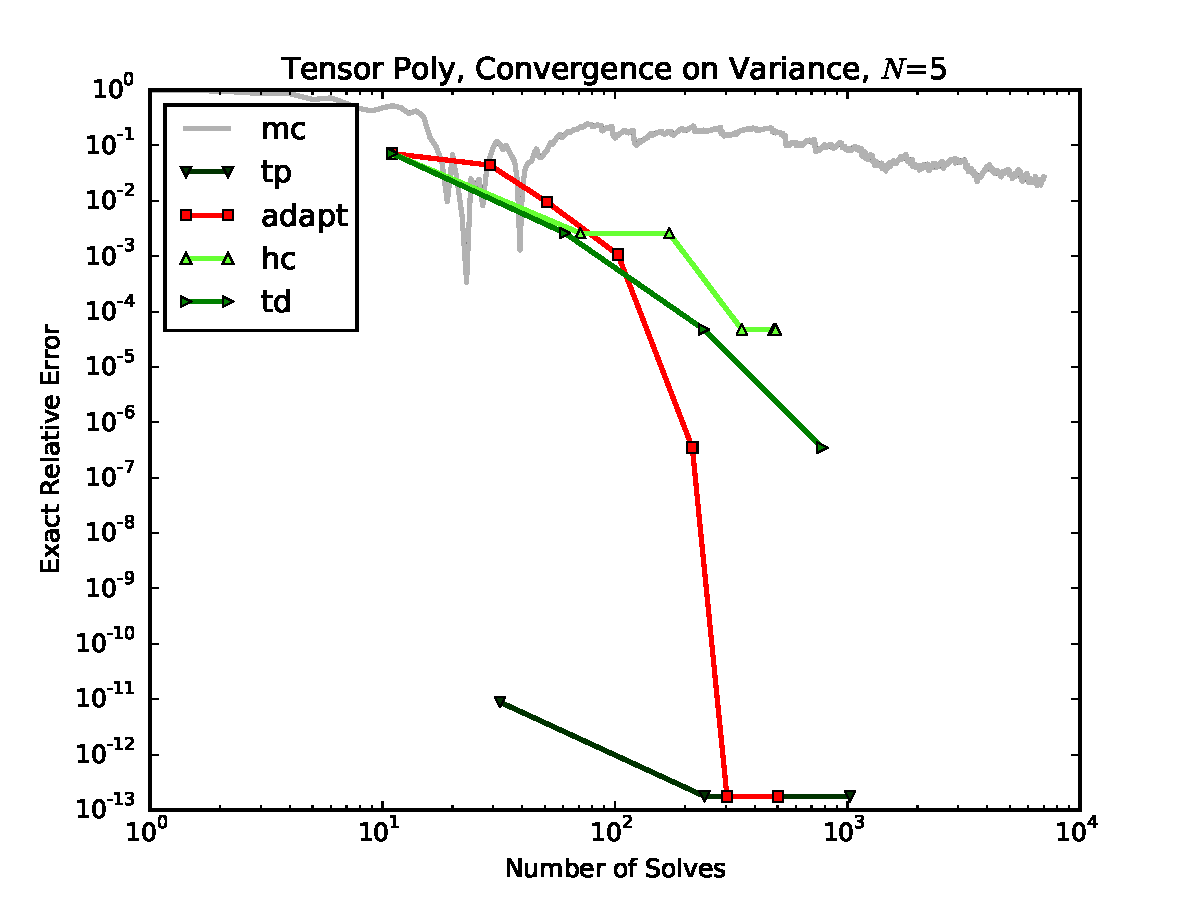
\includegraphics[width=\textwidth]{../../graphics/tenspoly_varconv_5}
    \end{figure}
  \end{column}
  \begin{column}{0.5\textwidth}
    \begin{figure}[h!]
      \centering
      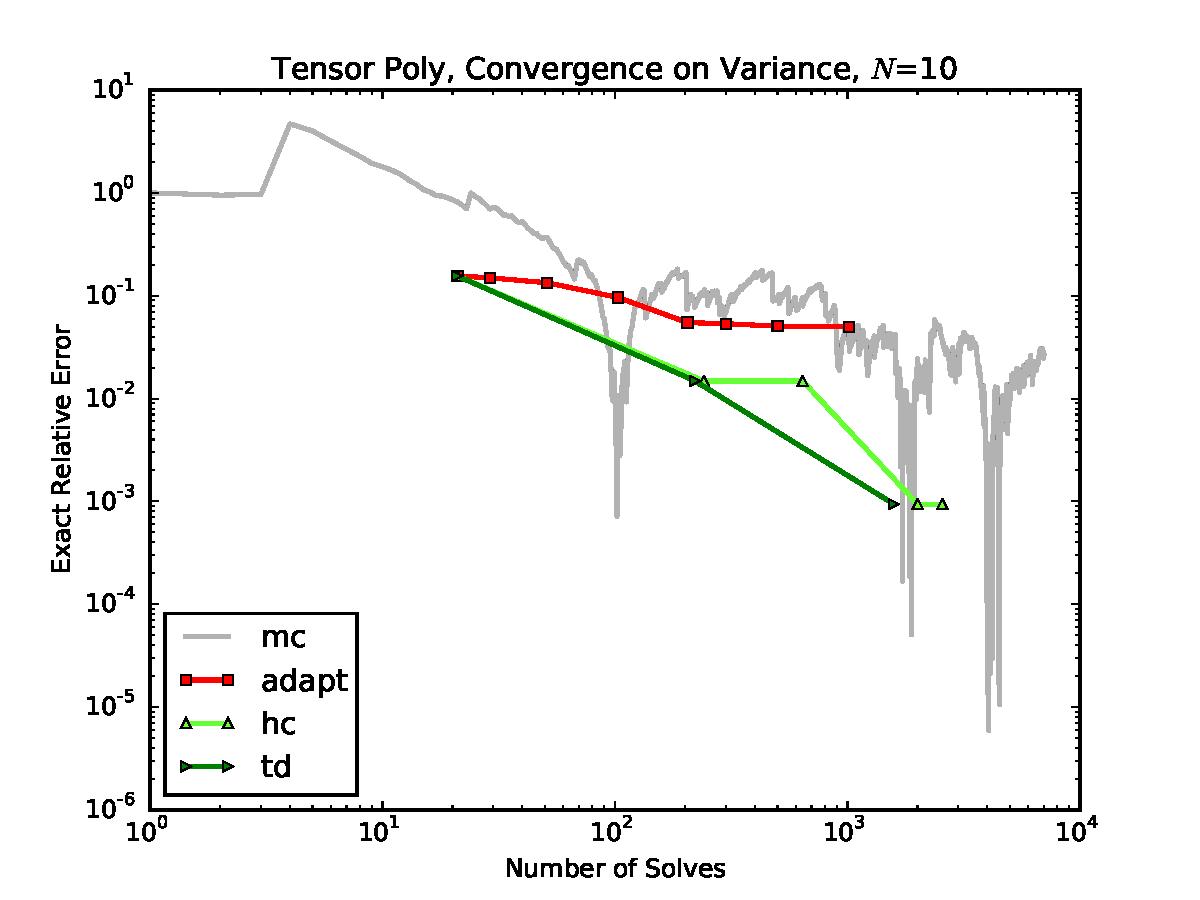
\includegraphics[width=\textwidth]{../../graphics/tenspoly_varconv_10}
    \end{figure}
  \end{column}
  \end{columns}
\end{frame}

\subsubsection{Attenuation}
\begin{frame}{Physical Models}{Attenuation}%\vspace{-20pt}
  Exit strength of beam incident on discrete absorbing material
  \begin{equation*}
    u(Y) = \prod_{n=1}^N e^{-y_n/N}, \hspace{10pt}y_n\sim\mathcal{U}[0,1]
  \end{equation*}
  Features:
  \begin{itemize}
    \item Analytic mean, variance
    \item Regularity
    \item Inexact in finite polynomial space
    \item Taylor expansion is tensor high-order polynomials
  \end{itemize}
\end{frame}

\begin{frame}{Attenuation}{Results}%\vspace{-20pt}
  \begin{columns}
  \begin{column}{0.5\textwidth}
    \begin{figure}[h!]
      \centering
      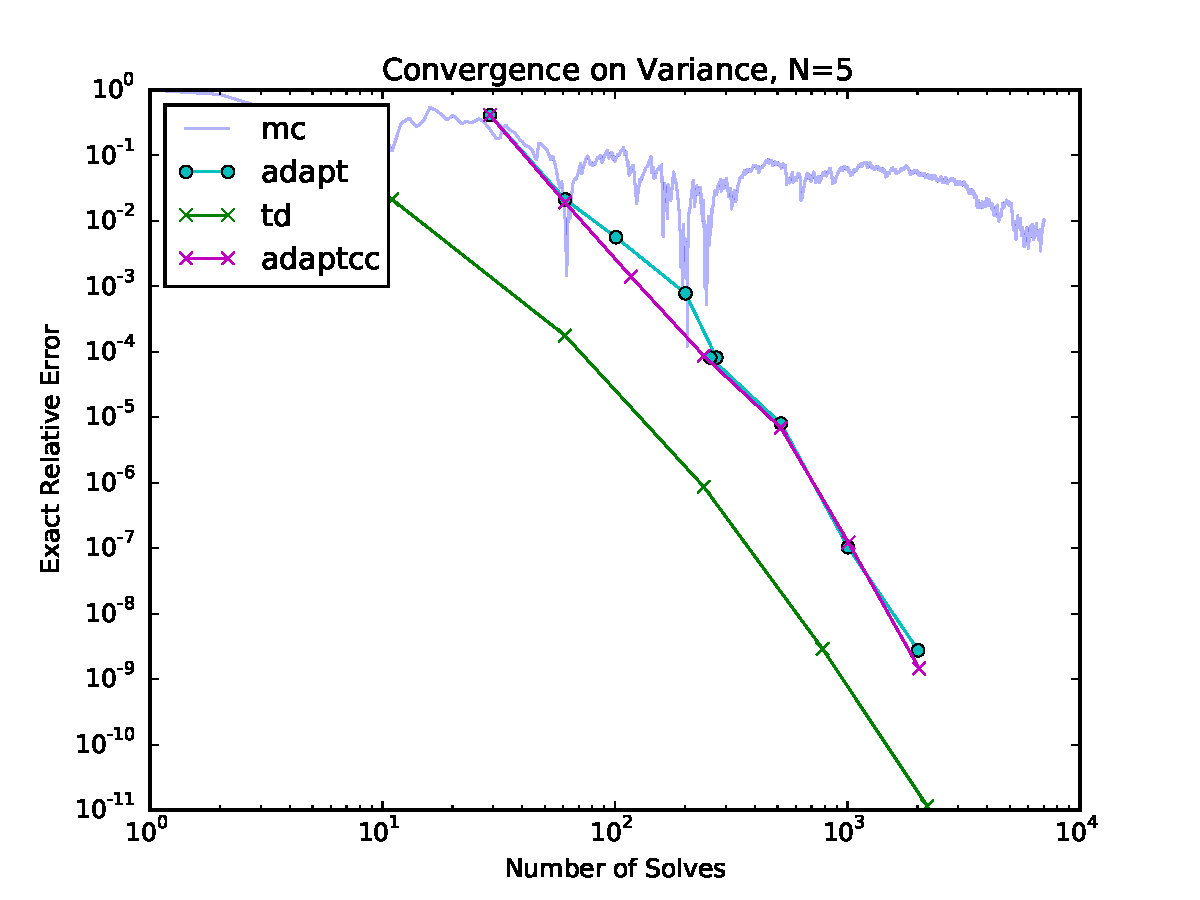
\includegraphics[width=\textwidth]{../../graphics/attn_varconv_5}
    \end{figure}
  \end{column}
  \begin{column}{0.5\textwidth}
    \begin{figure}[h!]
      \centering
      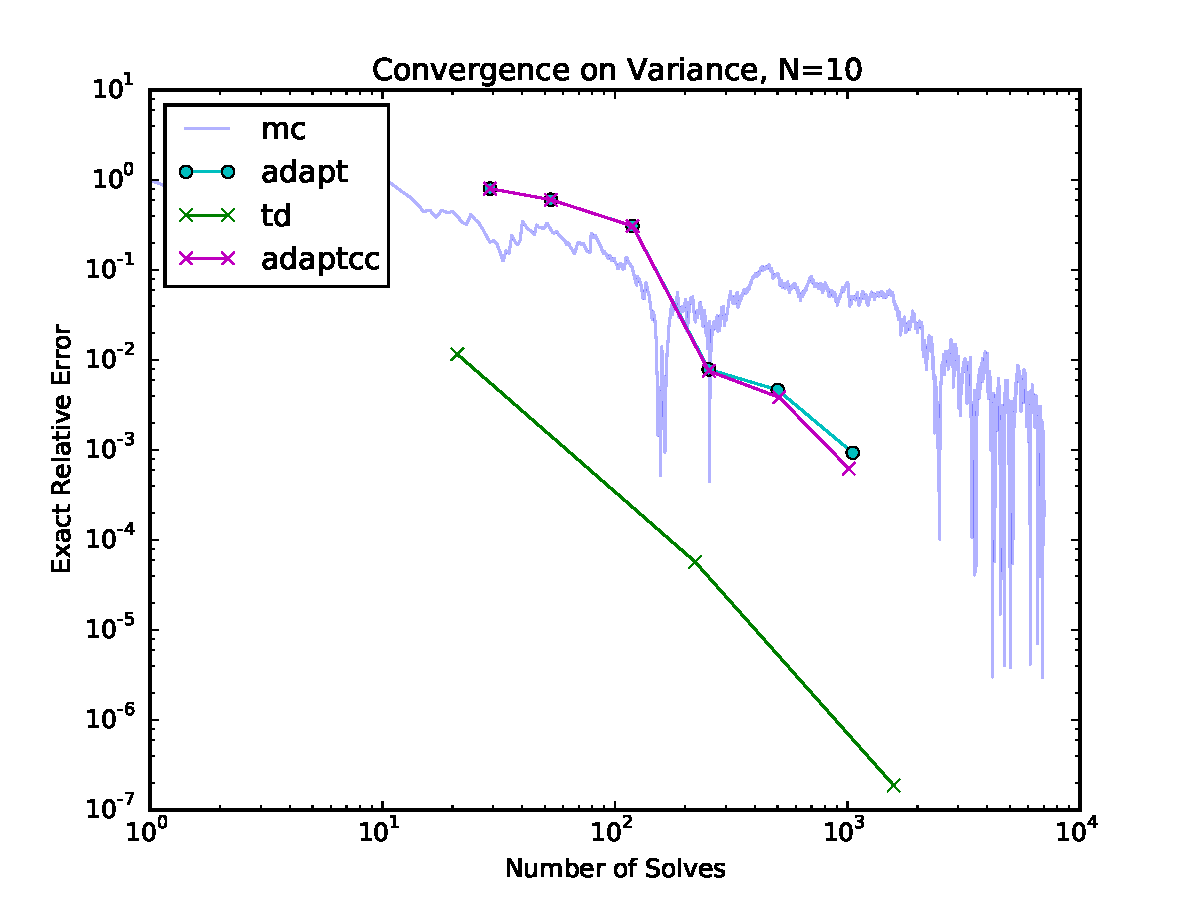
\includegraphics[width=\textwidth]{../../graphics/attn_varconv_10}
    \end{figure}
  \end{column}
  \end{columns}
\end{frame}


\subsubsection{Neutron Diffusion}
\begin{frame}{Physical Models}{Neutron Diffusion}\vspace{-20pt}
  Quarter-core 2-group steady state reactor benchmark \\165x165 cm domain 
  \footnotesize
  \begin{equation*}
    -\grad\cdot\qty( D_1(\bar x)\grad\phi_1(\bar x))+\qty(\xs{a}{1}(\bar x)+\xs{s}{1\to2}(\bar x))\phi_1(\bar x)
    = \frac{1}{k(\phi)}\sum_{g'=1}^2\nu_{g'}\xs{f}{g'}(\bar x)\phi_{g'}(\bar x),
  \end{equation*}
  \begin{equation*}
    -\grad \cdot\qty(D_2(\bar x)\grad \phi_2(\bar x))+\xs{a}{2}(\bar x)\phi_2(\bar x) = \xs{s}{1\to 2}(\bar
    x)\phi_1(\bar x)
  \end{equation*}
  QoI: $k(\phi)$
\end{frame}

\begin{frame}{Neutron Diffusion}{Geometry}%\vspace{-20pt}
  \begin{columns}
  \begin{column}{0.5\textwidth}
    \begin{figure}[h!]
      \centering
      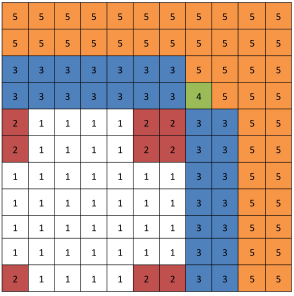
\includegraphics[width=0.5\textwidth]{../../graphics/core}
    \end{figure}
  \end{column}
  \begin{column}{0.5\textwidth}
    Vacuum, Reflective boundaries
  \end{column}
  \end{columns}
\end{frame}

\begin{frame}{Neutron Diffusion}{BCs}%\vspace{-20pt}
  Boundary Conditions
  \begin{equation}
    \frac{\phi_g}{4}-\frac{D_g}{2}\eval{\pdv{\phi_g}{x_1}}_{\partial \Omega_\text{top}}=0,\hspace{5pt} g=1,2,
  \end{equation}
  \begin{equation}
    \frac{\phi_g}{4}-\frac{D_g}{2}\eval{\pdv{\phi_g}{x_2}}_{\partial \Omega_\text{right}}=0,\hspace{5pt} g=1,2,
  \end{equation}
  \begin{equation}
    -D_g\eval{\pdv{\phi_g}{x_1}}_{\partial \Omega_\text{bottom}}=0,\hspace{5pt} g=1,2,
  \end{equation}
  \begin{equation}
    -D_g\eval{\pdv{\phi_g}{x_2}}_{\partial \Omega_\text{left}}=0,\hspace{5pt} g=1,2.
  \end{equation}
\end{frame}

\begin{frame}{Neutron Diffusion}{Input Space}%\vspace{-20pt}
  \begin{table}[h]
    \centering
    \begin{tabular}{c c | c c c c}
      Region & Group & $D_g$ & $\Sigma_{a,g}$ & $\nu\Sigma_{f,g}$ & $\Sigma_s^{1,2}$ \\ \hline
      1 & 1 & 1.255 & 8.252e-3 & 4.602e-3 & 2.533e-2 \\
       & 2 & 2.11e-1 & 1.003e-1 & 1.091e-1 & \\ \hline
       2 & 1 & 1.268 & 7.181e-3 & 4.609e-3 & 2.767e-2 \\
        & 2 & 1.902e-1 & 7.047e-2 & 8.675e-2 & \\ \hline
        3 & 1 & 1.259 & 8.002e-3 & 4.663e-3 & 2.617e-2 \\
         & 2 & 2.091e-1 & 8.344e-2 & 1.021e-1 & \\ \hline
         4 & 1 & 1.259 & 8.002e-3 & 4.663e-3 & 2.617e-2 \\
          & 2 & 2.091e-1 & 7.3324e-2 & 1.021e-1 & \\ \hline
          5 & 1 & 1.257 & 6.034e-4 & 0 & 4.754e-2 \\
           & 2 & 1.592e-1 & 1.911e-2 & 0 &
         \end{tabular}
         %\caption{Reference Material Properties for Benchmark Core}
         %\label{tab:coremats}
       \end{table}
\end{frame}

\begin{frame}{Neutron Diffusion}{Reference Solution}%\vspace{-20pt}
  $k$=1.00007605445
  \begin{columns}
  \begin{column}{0.5\textwidth}
  \begin{figure}[h!]
    \centering
    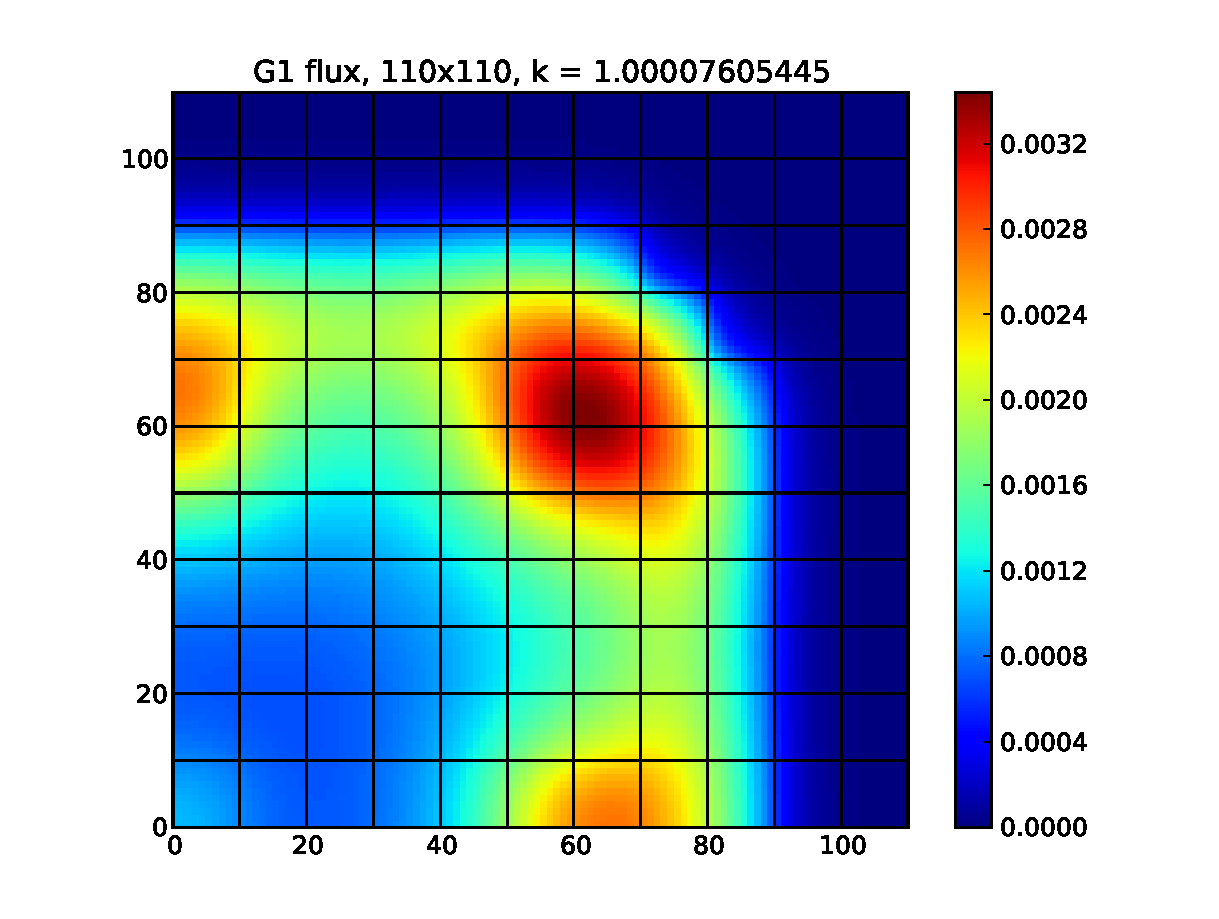
\includegraphics[width=\textwidth]{../../graphics/g1_50_flux}
  \end{figure}
  \end{column}
  \begin{column}{0.5\textwidth}
  \begin{figure}[h!]
    \centering
    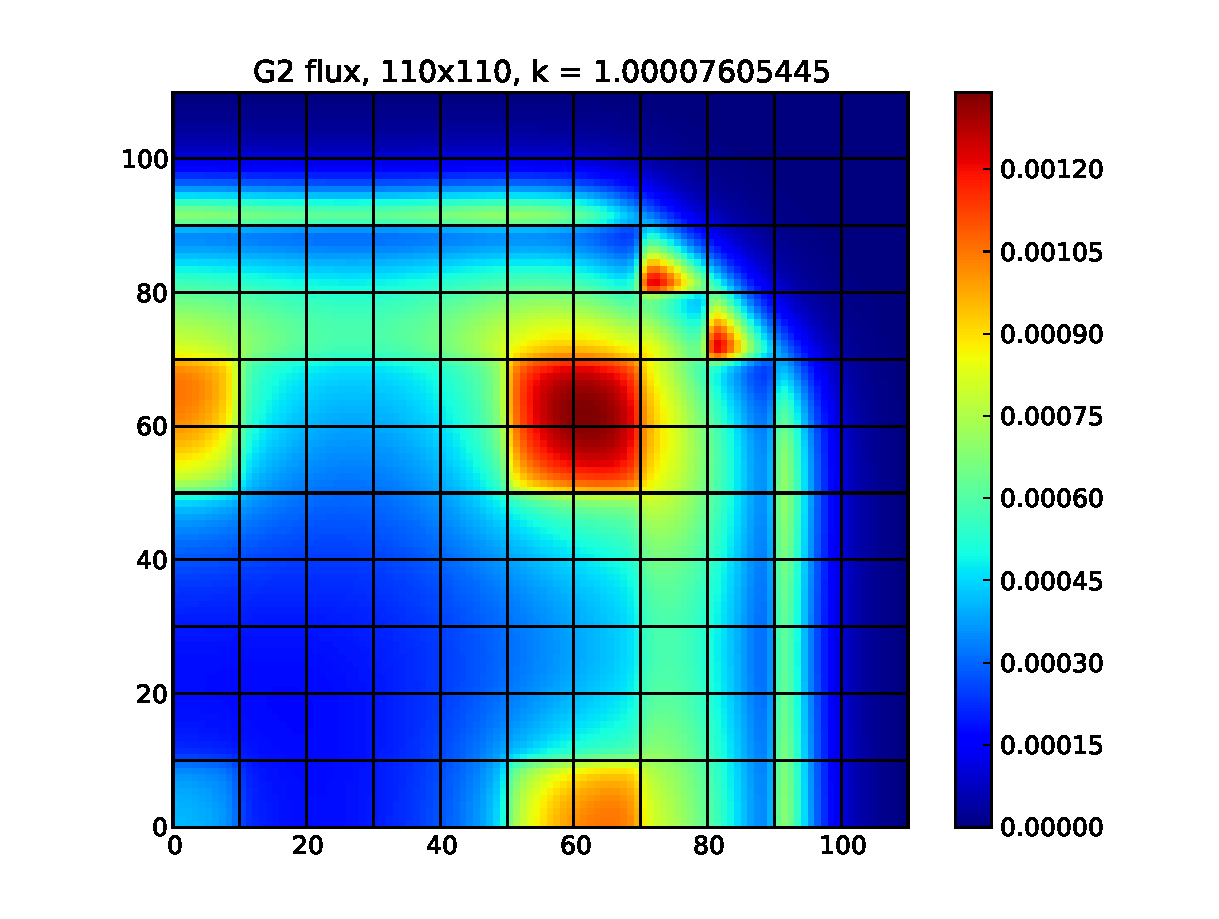
\includegraphics[width=\textwidth]{../../graphics/g2_50_flux}
  \end{figure}
  \end{column}
  \end{columns}
\end{frame}

\begin{frame}{Neutron Diffusion}{Uncertainty}\vspace{-20pt}
  5\% Uncertainty in Parameters:
  \begin{columns}
  \begin{column}{0.5\textwidth}
    $N$=3, $N$=5
    \begin{itemize}
      \item $\nu\Sigma^{(1)}_{2,f}$
      \item $\nu\Sigma^{(4)}_{2,f}$
      \item $D^{(5)}_2$ \vspace{20pt}
      \item $\Sigma^{(1)}_{2,c}$
      \item $\Sigma^{(4)}_{2,c}$
    \end{itemize}
  \end{column}
  \begin{column}{0.5\textwidth}
    $N$=10
    \begin{itemize}
      \item $\Sigma^{(1)}_{2,c}$, $\nu\Sigma^{(1)}_{2,f}$
      \item $\Sigma^{(2)}_{2,c}$, $\nu\Sigma^{(2)}_{2,f}$
      \item $\Sigma^{(3)}_{2,c}$, $\nu\Sigma^{(3)}_{2,f}$
      \item $\Sigma^{(4)}_{2,c}$, $\nu\Sigma^{(4)}_{2,f}$, $\nu\Sigma^{(4)}_{1\to2}$
      \item $D^{(5)}_2$ \vspace{20pt}
    \end{itemize}
  \end{column}
  \end{columns}
\end{frame}

\begin{frame}{Neutron Diffusion}{Results}%\vspace{-20pt}
  $N$=3
  \begin{figure}[h!]
    \centering
    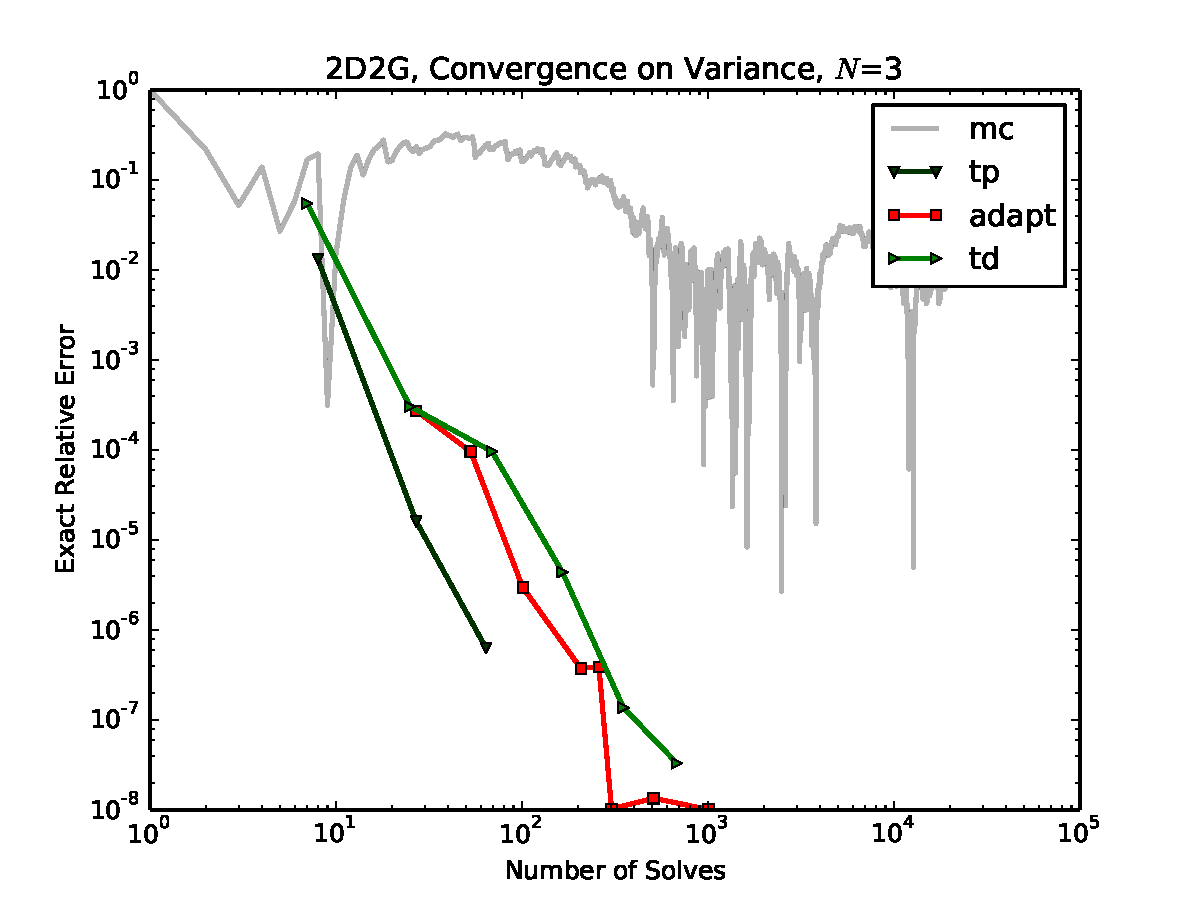
\includegraphics[width=0.7\textwidth]{../../graphics/2D2G_varconv_3}
  \end{figure}
\end{frame}

\begin{frame}{Neutron Diffusion}{Results}%\vspace{-20pt}
  $N$=5
  \begin{figure}[h!]
    \centering
    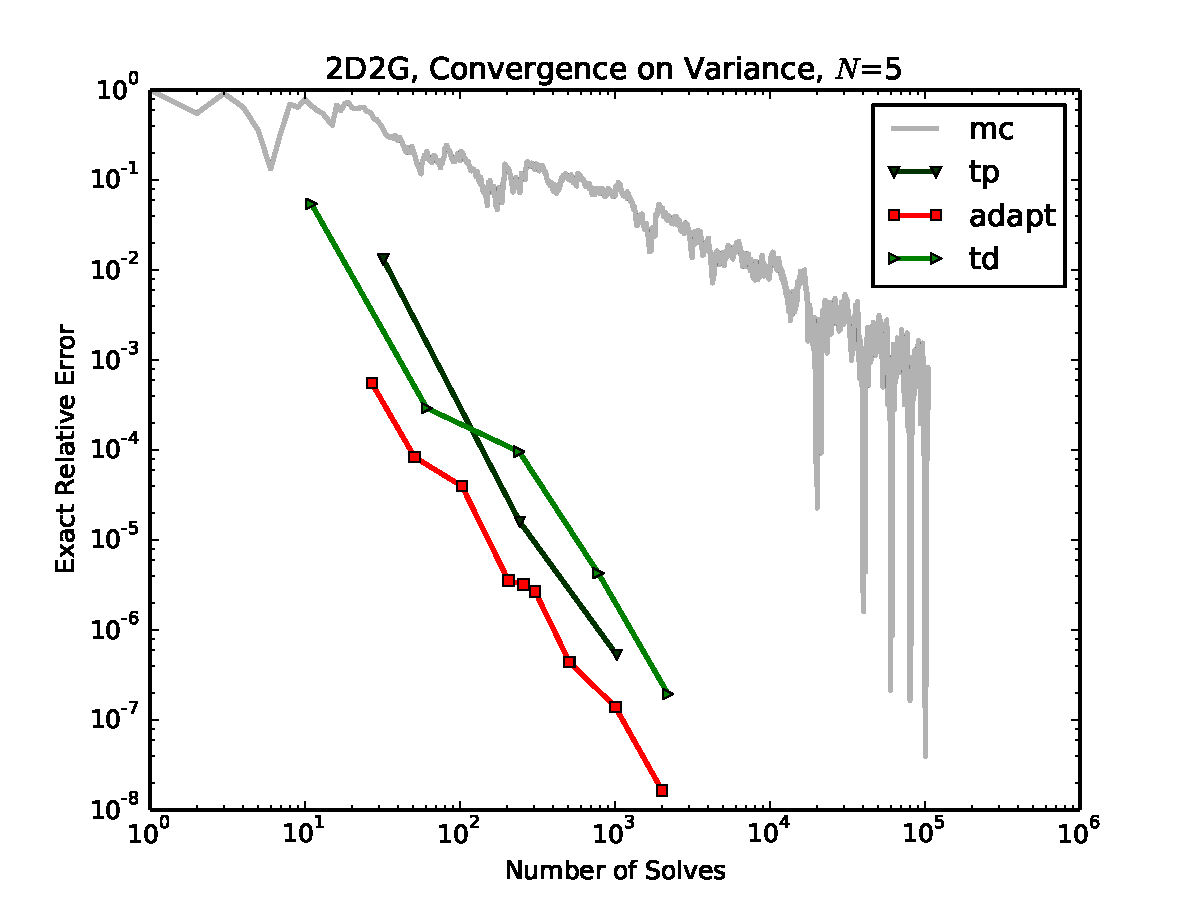
\includegraphics[width=0.7\textwidth]{../../graphics/2D2G_varconv_5}
  \end{figure}
\end{frame}

\begin{frame}{Neutron Diffusion}{Results}%\vspace{-20pt}
  $N$=10
  \begin{figure}[h!]
    \centering
    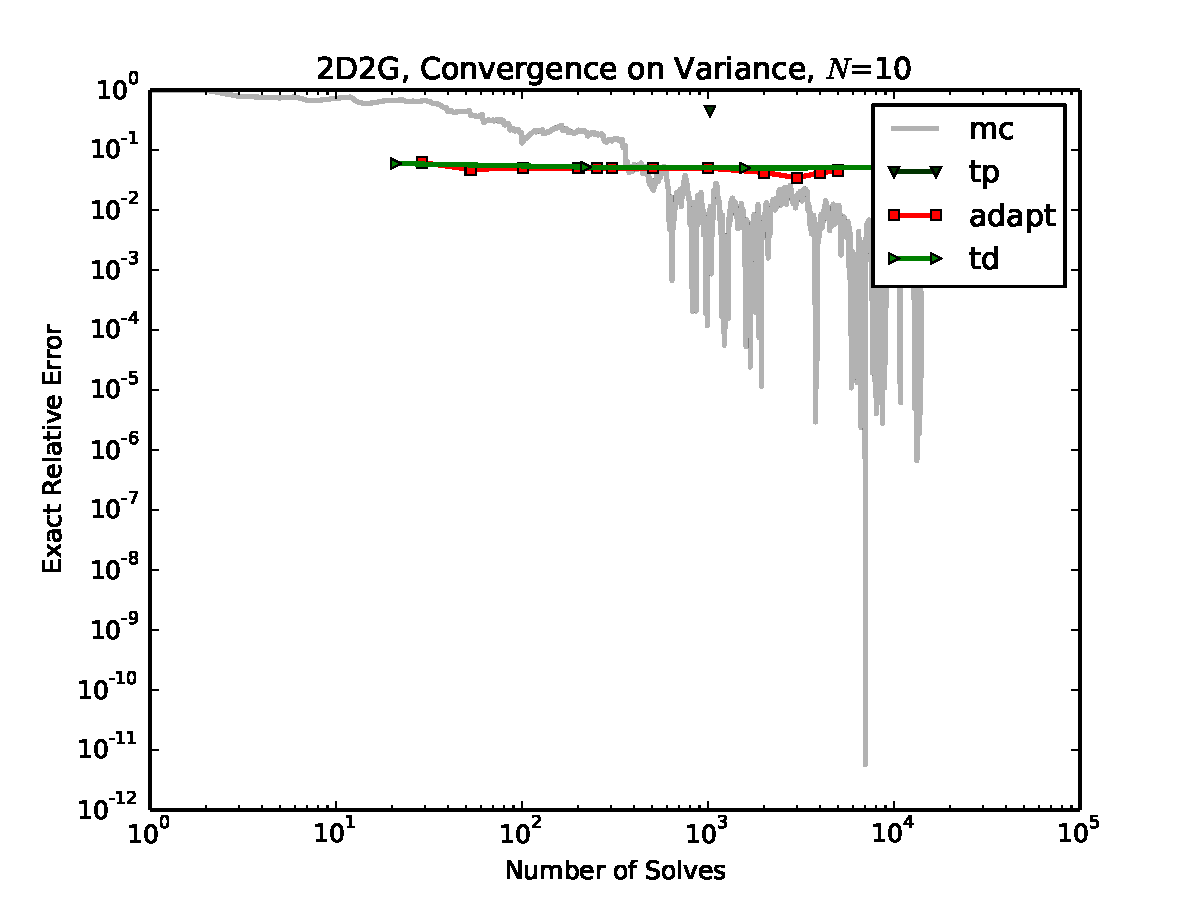
\includegraphics[width=0.7\textwidth]{../../graphics/2D2G_varconv_10}
  \end{figure}
\end{frame}

\begin{frame}{Neutron Diffusion}{Results}\vspace{-20pt}
  \begin{columns}
  \begin{column}{0.3\textwidth}
    \begin{figure}[h!]
      \centering
      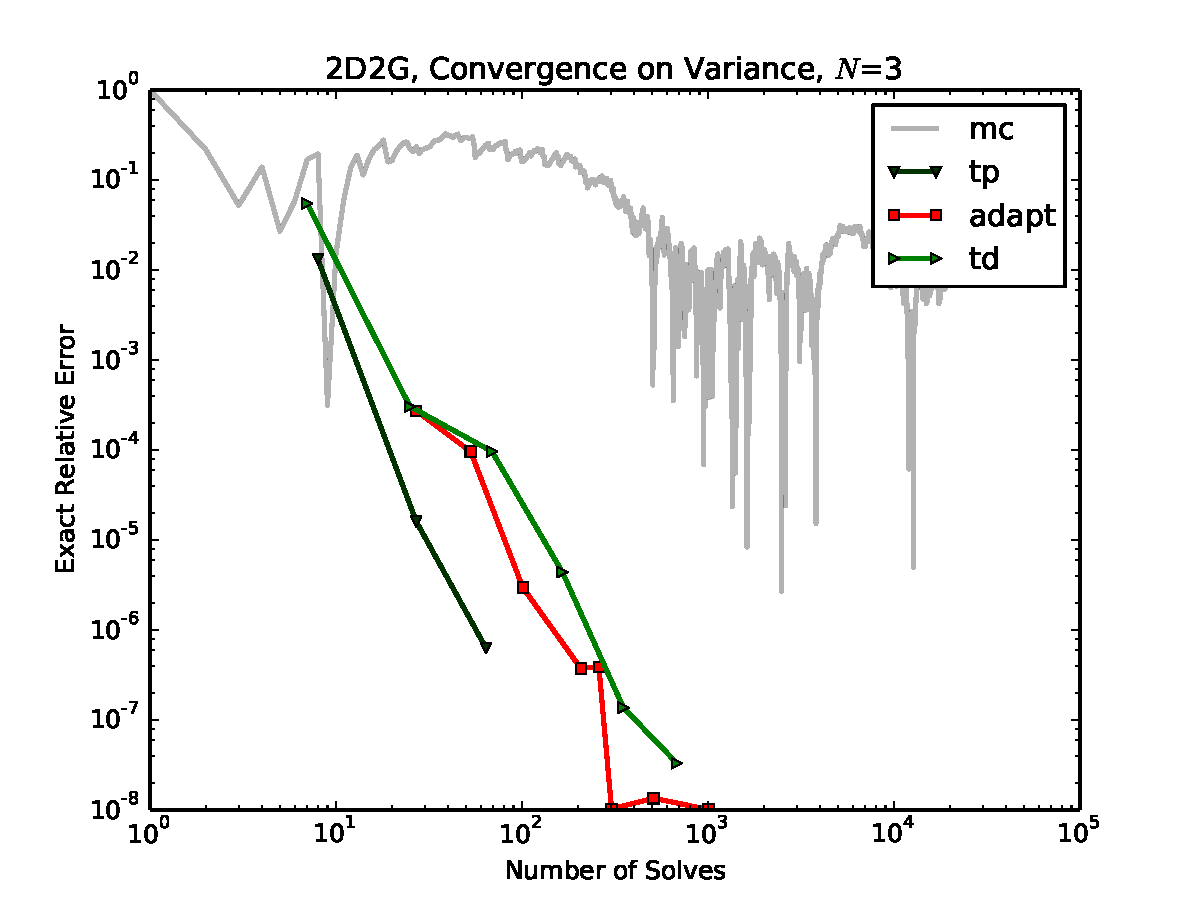
\includegraphics[width=\textwidth]{../../graphics/2D2G_varconv_3}
    \end{figure}
  \end{column}
  \begin{column}{0.3\textwidth}
    \begin{figure}[h!]
      \centering
      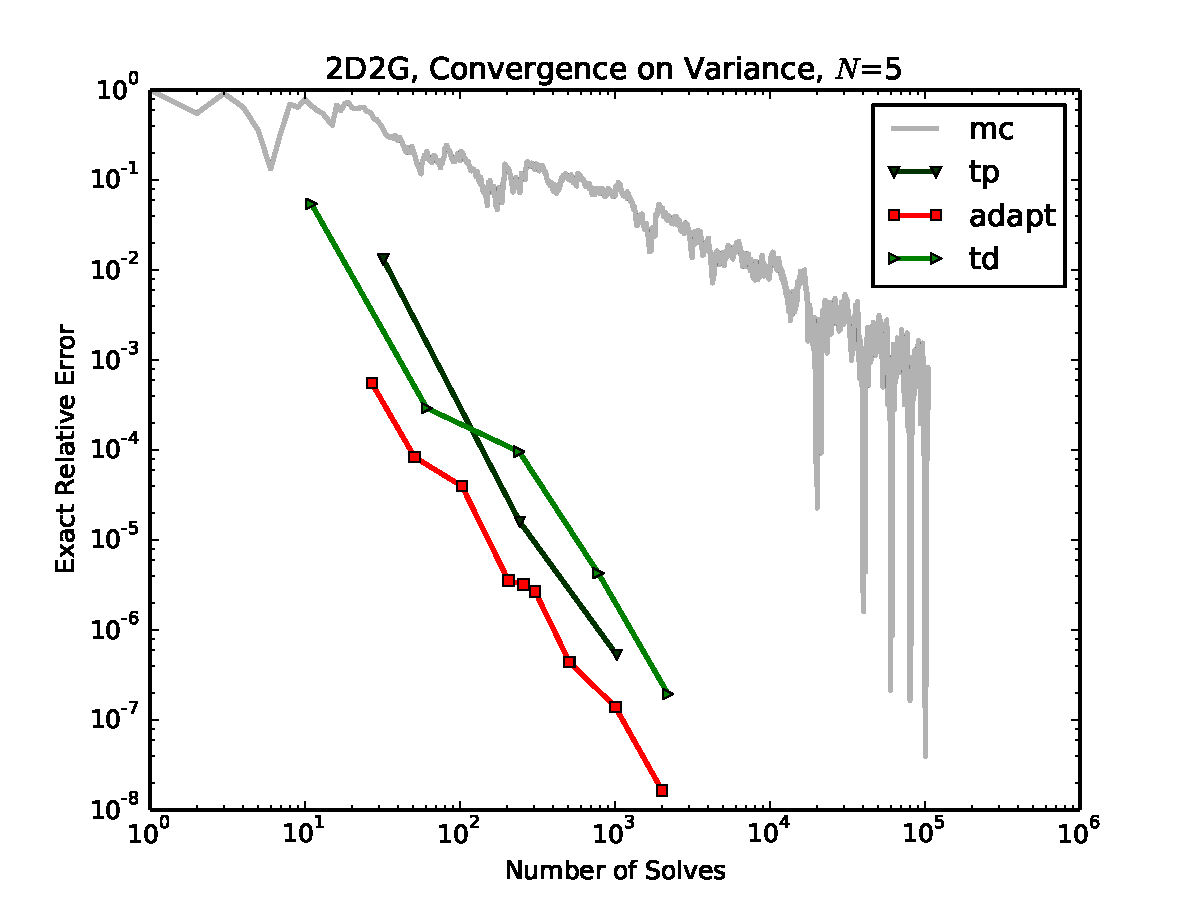
\includegraphics[width=\textwidth]{../../graphics/2D2G_varconv_5}
    \end{figure}
  \end{column}
  \begin{column}{0.3\textwidth}
    \begin{figure}[h!]
      \centering
      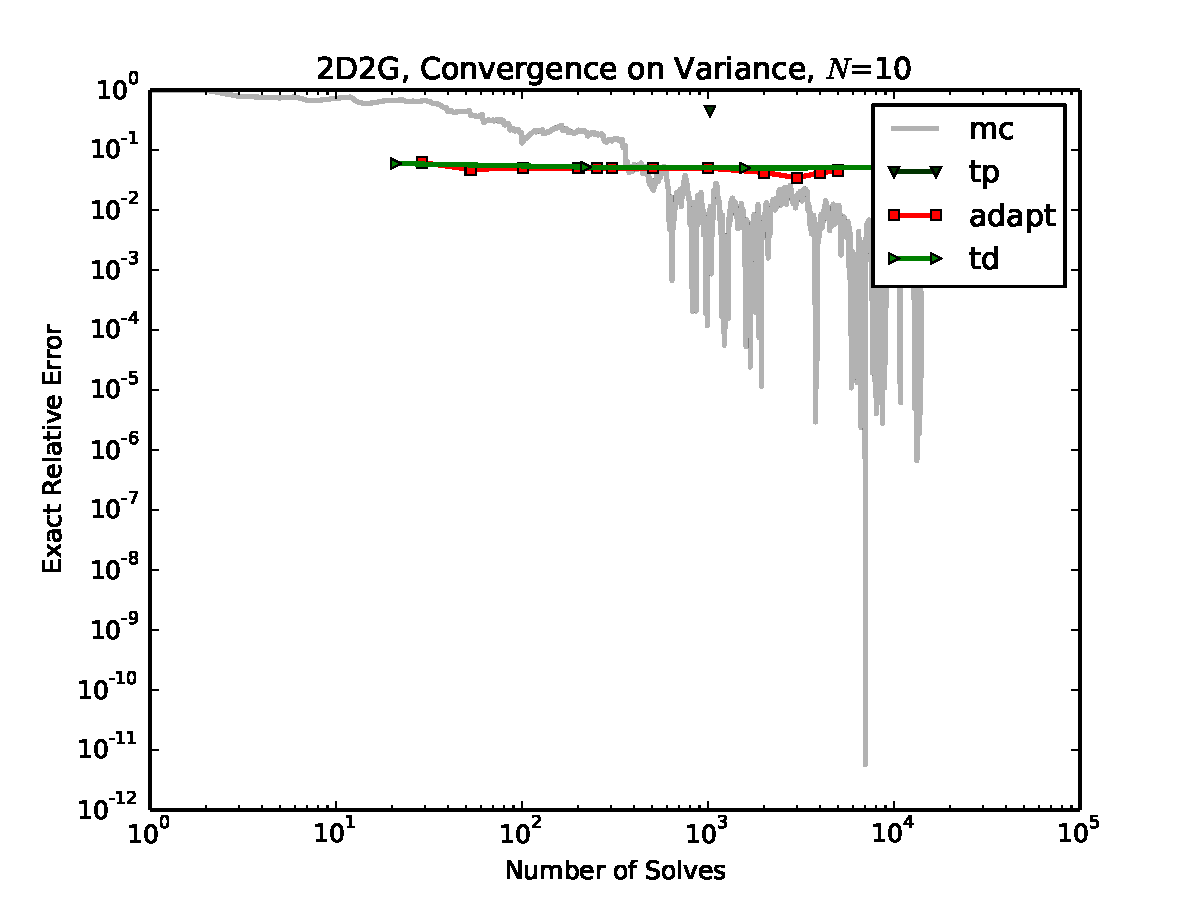
\includegraphics[width=\textwidth]{../../graphics/2D2G_varconv_10}
    \end{figure}
  \end{column}
  \end{columns}
\end{frame}

\begin{frame}{Results}{Summary}\vspace{-20pt}
  Preliminary Conclusions\vspace{20pt}
  \begin{itemize}
    \item SC for gPC suffers greatly from curse of dimensionality\vspace{10pt}
    \item Adaptive SC can help\vspace{10pt}
    \item For 5 or less dimensions, performs well for regular responses
  \end{itemize}
\end{frame}

%%%%%%%%%%%%%%%%%%%%%%%%%%%%
%        PROPOSAL          % 15-20 minutes
%%%%%%%%%%%%%%%%%%%%%%%%%%%%
\section{Proposal}

\subsection{HDMR}
\begin{frame}{Proposal}{HDMR}\vspace{-20pt}
  ANOVA method to decompose input space
  \begin{equation*}
  \tilde H[u](Y) = u_0 + \sum_{i=1}^N u_i + \sum_{i_1=1}^N\sum_{i_2=1}^{i_1-1}u_{ij}+\cdots +
      u_{i_1,\ldots,i_N},
  \end{equation*}
  \begin{align*}
    u_0 \equiv& \int dy_1\cdots\int dy_N u(Y), \\
    u_i \equiv& \int dy_1\cdots\int dy_{i-1}\int dy_{i+1}\cdots\int dy_N u(Y) - u_0
  \end{align*}
\end{frame}

\begin{frame}{Proposal}{HDMR}\vspace{-20pt}
  Sobol' sensitivity coefficients
  \begin{equation*}
    \mathcal{S}_i = \frac{\text{var}\left\{u_i\right\}}{\text{var}\left\{\tilde H[u](Y)\right\}}
  \end{equation*}
  \begin{equation*}
    \text{var}\left\{u(Y)\right\}= \sum_{i=1}^N \mathcal{S}_i + \sum_{i_1=1}^N\sum_{i_2=1}^{i_1-1}
    \mathcal{S}_{ij}+\cdots+\mathcal{S}_{i_1,\ldots,i_N}
  \end{equation*}
\end{frame}

\begin{frame}{Proposal}{HDMR}%\vspace{-20pt}
  Problem: Costly integrals (even low-level expansion)\\
  Solution: Cut-HDMR, reference point $\hat Y=(\hat y_1,\ldots,\hat y_N)$\\
  Let $u(y_i) \equiv u(\hat y_1,\ldots,\hat y_{i-1},\hspace{5pt}y_i\hspace{5pt},\hat y_{i+1},\ldots,\hat y_N)$
  \begin{equation*}
  H[u](Y) = h_0 + \sum_{i=1}^N h_i + \sum_{i_1=1}^N\sum_{i_2=1}^{i_1-1}h_{ij}+\cdots +
      h_{i_1,\ldots,i_N},
  \end{equation*}
  \begin{align*}
    h_0 \equiv& u(\hat Y), \\
    h_i \equiv& u(y_i) - h_0, \\
    h_{ij} \equiv& u(y_i,y_j) -h_i - h_j - h_0
  \end{align*}
\end{frame}

\begin{frame}{Proposal}{HDMR}\vspace{-20pt}
  Problem with Cut-HDMR: Terms not orthogonal
  \begin{equation*}
    \mathcal{S}_i \neq \frac{\text{var}\left\{h_i\right\}}{\text{var}\left\{H[u](Y)\right\}}\equiv\xi_{ij} 
  \end{equation*}
  \begin{equation*}
    \text{var}\left\{u(Y)\right\}\neq \sum_{i=1}^N \xi_i + \sum_{i_1=1}^N\sum_{i_2=1}^{i_1-1}
         \xi_{ij}+\cdots+\xi_{i_1,\ldots,i_N}
  \end{equation*}
  However, no integrals!
\end{frame}

\begin{frame}{Proposal}{HDMR}\vspace{-20pt}
  Next step: HDMR terms are SCgPC
  \begin{equation*}
  H[u](Y) = h_0 + \sum_{i=1}^N h_i + \sum_{i_1=1}^N\sum_{i_2=1}^{i_1-1}h_{ij}+\cdots +
      h_{i_1,\ldots,i_N},
  \end{equation*}
  \begin{align*}
    h_0 \equiv& u(\hat Y), \\
    h_i \equiv& G[u](y_i) - h_0, \\
    h_{ij} \equiv& G[u](y_i,y_j) -h_i - h_j - h_0
  \end{align*}
  Benefit: most terms low dimension, regular
\end{frame}

\subsection{Adaptive HDMR}
\begin{frame}{Proposal}{Adaptive HDMR}\vspace{-20pt}
  Better than HDMR: Adaptive HDMR with Adaptive SCgPC\\
  Choose terms based on impact parameters $\xi$, $\eta$
\begin{itemize}
  \item Evaluate the reference (all mean) case.
  \item Construct all HDMR first-order SCgPC models.
  \item While not converged:
  \begin{itemize}
    \item Using existing subset impacts, predict importance of future subsets
    \item Consider impact of adding polynomials to existing subset gPCs
    \item Choose: expand existing subsets or add new subsets
    \item If contribution of new HDMR expectation less than tolerance, convergence
  \end{itemize}
\end{itemize}
\end{frame}

\begin{frame}{Proposal}{Adaptive HDMR}\vspace{-20pt}
  Example, $N=3$
\begin{table}[h!]\footnotesize
\centering
\begin{tabular}{c c c c c c c c c c c c c c c c c}
    $H[u](Y)$ &$=$ &$h_0$ $+$ &$h_1$ $+$ &$h_2$ $+$ &$h_3$ $+$ &$h_{12}$ $+$ &$h_{13}$ $+$ &$h_{23}$ $+$
    &$h_{123}$ \\\hline
              &    & 0        & 1        & 1        & 1        &             &             &             & \\     
SCgPC Order:  &    & 0        & 2        & 1        & 1        &             &             &             & \\     
              &    & 0        & 2        & 1        & 1        & (1,1)       &             &             & \\     
              &    & 0        & 2        & 2        & 1        & (1,1)       &             &             & \\     
              &    & 0        & 2        & 2        & 1        & (1,2)       &             &             & \\     
              &    & 0        & 2        & 2        & 2        & (1,2)       &             &             &      
\end{tabular}
\end{table}
%  \begin{align*}
%    H[u](Y) = &h_0 + & h_1 + & h_2 + & h_3 + & h_{12} + & h_{13} + & h_{23} + & h_{123} \\
%\text{Poly Order: } & 0 & 1 & 1    & 1    &         &         &         &  \\
%                    & 0 & 1 & 2    & 1    &         &         &         &  \\
%                    & 0 & 1 & 2    & 1    & 1       &         &         &  \\
%                    & 0 & 1 & 2    & 1    & 1       & 1       &         & 
%  \end{align*}
\end{frame}

\subsection{Mammoth}
\begin{frame}{Proposal}{Mammoth}\vspace{-20pt}
  \begin{columns}
  \begin{column}{0.7\linewidth}
  Mammoth: MOOSE framework MultiApp
  \end{column}
  \begin{column}{0.3\linewidth}
    \begin{figure}[h!]
      \centering
      
\includegraphics[width=\textwidth]{../../graphics/moose_multiphysics}
    \end{figure}
  \end{column}
  \end{columns}
  \begin{itemize}
    \item RattleS$_\text{N}$ake: Neutron Transport code
      \begin{itemize}
        \item Provides power distributions
        \item Tens of thousands of inputs
      \end{itemize}
    \item Bison: Fuel Performance code
      \begin{itemize}
        \item Analyzes fuel: stress, temperature, displacement
        \item Dozens of inputs
      \end{itemize}
  \end{itemize}
  \vspace{10pt}
  Goal: Demonstrate Adaptive HDMR with Adaptive SCgPC
\end{frame}

\begin{frame}{Proposal}{Special Thanks}\vspace{-20pt}
  \pause
  Dept. Nuclear Engineering, UNM
  \begin{itemize}
    \item Dr. Anil Prinja, Adviser and Chair
    \item Aaron Olsen, Peer
  \end{itemize}
  RAVEN team, Idaho National Laboratory
  \begin{itemize}
    \item Dr. Cristian Rabiti, Manager and Mentor
    \item Andrea Alfonsi, Mentor
    \item Daniel Maljovec, Peer
  \end{itemize}
  \vspace{10pt}
  \centering
  Research performed under LDRD grant through Idaho National Laboratory
\end{frame}

\end{document}






